\section{\textcolor{red}{Splay Tree}}
\section{Estructura de la Implementación}
La implementación se divide en varias partes: la definición de los nodos del árbol, las operaciones básicas del Splay Tree (inserción, eliminación, splay, etc.) y la representación gráfica utilizando GraphStream.

\subsection{Definición de la Clase Nodo}
La clase \mj{TreeNode} es una clase estática anidada dentro de la clase \mj{SplayTree}. Esta clase representa los nodos del árbol.
\begin{minted}[bgcolor=background]{java}
private static class TreeNode<T> {
  T key;
  TreeNode<T> left, right;

  TreeNode(T key) {
    this.key = key;
    this.left = this.right = null;
  }
}
\end{minted}

\subsection{Operaciones Básicas del Splay Tree}
La clase \mj{SplayTree} implementa las operaciones básicas de un Splay Tree como inserción, eliminación, búsqueda y la operación de splay. A continuación, se describen algunos de estos métodos:

\subsubsection{Método Insert}
El método \mj{insert} añade un nuevo nodo al árbol y luego aplica la operación de splay para mover dicho nodo a la raíz.
\begin{minted}[bgcolor=background]{java}
@Override
public void insert(T key) {
  root = insert(root, key);
  splay(key);
}

private TreeNode<T> insert(TreeNode<T> node, T key) {
  if (node == null) {
    return new TreeNode<>(key);
  }
  int cmp = key.compareTo(node.key);
  if (cmp < 0) {
    node.left = insert(node.left, key);
  } else if (cmp > 0) {
    node.right = insert(node.right, key);
  }
  return node;
}
\end{minted}

\subsubsection{Método Splay}
El método \mj{splay} mueve el nodo con la clave especificada a la raíz del árbol. Esta operación mejora el rendimiento de futuras operaciones en el nodo accedido.
\begin{minted}[bgcolor=background]{java}
@Override
public void splay(T key) {
  root = splay(root, key);
}

private TreeNode<T> splay(TreeNode<T> node, T key) {
  if (node == null) return null;

  int cmp1 = key.compareTo(node.key);
  if (cmp1 < 0) {
    if (node.left == null) return node;
    int cmp2 = key.compareTo(node.left.key);
    if (cmp2 < 0) {
      node.left.left = splay(node.left.left, key);
      node = rotateRight(node);
    } else if (cmp2 > 0) {
      node.left.right = splay(node.left.right, key);
      if (node.left.right != null) {
        node.left = rotateLeft(node.left);
      }
    }
    return node.left == null ? node : rotateRight(node);
  } else if (cmp1 > 0) {
    if (node.right == null) return node;
    int cmp2 = key.compareTo(node.right.key);
    if (cmp2 < 0) {
      node.right.left = splay(node.right.left, key);
      if (node.right.left != null) {
        node.right = rotateRight(node.right);
      }
    } else if (cmp2 > 0) {
      node.right.right = splay(node.right.right, key);
      node = rotateLeft(node);
    }
    return node.right == null ? node : rotateLeft(node);
  } else {
    return node;
  }
}
\end{minted}

\subsubsection{Rotaciones}
Las rotaciones son operaciones auxiliares utilizadas durante la operación de splay para reestructurar el árbol. Las siguientes son las implementaciones de rotación a la derecha e izquierda:
\begin{minted}[bgcolor=background]{java}
private TreeNode<T> rotateRight(TreeNode<T> node) {
  TreeNode<T> temp = node.left;
  node.left = temp.right;
  temp.right = node;
  return temp;
}

private TreeNode<T> rotateLeft(TreeNode<T> node) {
  TreeNode<T> temp = node.right;
  node.right = temp.left;
  temp.left = node;
  return temp;
}
\end{minted}

\subsection{Representación Gráfica con GraphStream}
La clase \mj{SplayTree} también incluye un método para representar gráficamente el árbol utilizando la librería GraphStream. Este método agrega los nodos y las aristas al grafo y lo muestra visualmente.

\subsubsection{Método DisplayTree}
El método \mj{displayTree} inicializa el grafo y llama al método \mj{addNodesAndEdges} para agregar los nodos y las aristas.
\begin{minted}[bgcolor=background]{java}
public void displayTree() {
  System.setProperty("org.graphstream.ui", "swing");
  Graph graph = new SingleGraph("Splay Tree");

  addNodesAndEdges(graph, root);

  for (Node node : graph) {
    node.setAttribute("ui.label", node.getId());
  }

  graph.display();
}
\end{minted}

\subsubsection{Método AddNodesAndEdges}
El método \mj{addNodesAndEdges} es responsable de agregar los nodos y las aristas al grafo. Para evitar la duplicación de código, se utilizan los métodos auxiliares \mj{addNode} y \mj{addEdge}:
\begin{minted}[bgcolor=background]{java}
private void addNodesAndEdges(Graph graph, TreeNode<T> node) {
  if (node == null) return;

  addNode(graph, node.key.toString());

  if (node.left != null) {
    addNode(graph, node.left.key.toString());
    addEdge(graph, node.key.toString(), node.left.key.toString());
    addNodesAndEdges(graph, node.left);
  }

  if (node.right != null) {
    addNode(graph, node.right.key.toString());
    addEdge(graph, node.key.toString(), node.right.key.toString());
    addNodesAndEdges(graph, node.right);
  }
}

private void addNode(Graph graph, String key) {
  if (graph.getNode(key) == null) {
    graph.addNode(key);
  }
}

private void addEdge(Graph graph, String parentKey, String childKey) {
  String edgeId = parentKey + "-" + childKey;
  if (graph.getEdge(edgeId) == null) {
    graph.addEdge(edgeId, parentKey, childKey, true);
  }
}
\end{minted}

\section{Visualización}
Esta representación gráfica es útil para entender el comportamiento del Splay Tree y cómo las operaciones de splay mejoran el rendimiento del árbol.

\begin{minted}{zsh}
$ javac -cp .:jar/gs-algo-2.0.jar:jar/gs-core-2.0.jar:jar/gs-ui-swing-2.0.jar TestSplayTree.java
$ java -cp .:jar/gs-algo-2.0.jar:jar/gs-core-2.0.jar:jar/gs-ui-swing-2.0.jar TestSplayTree
10 20 25 30 40 50
\end{minted}

\begin{figure}[H]
  \centering
  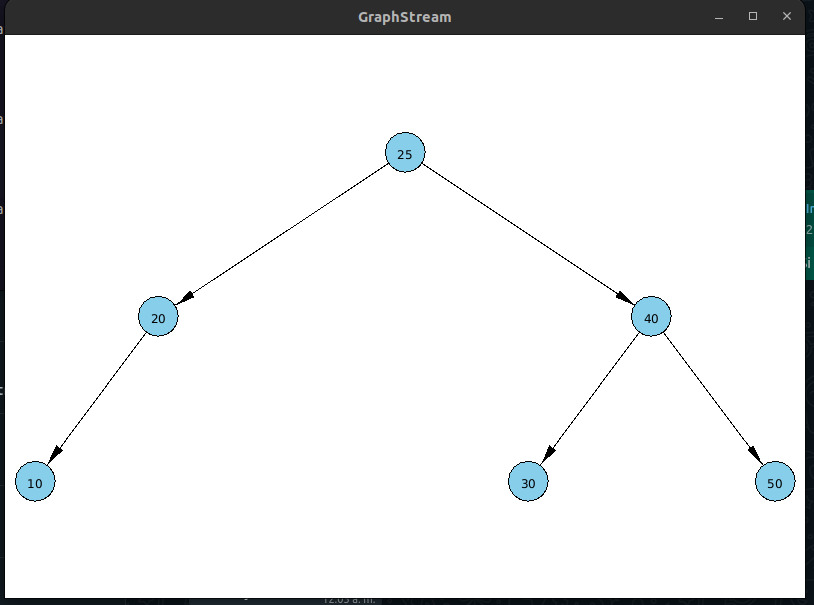
\includegraphics[width=0.7\textwidth]{img/representation_splayTree.png}
  \caption{Splay Tree}
\end{figure}

